% Triángulo ideal: vértices en la frontera y lados geodésicos ortogonales a ella.
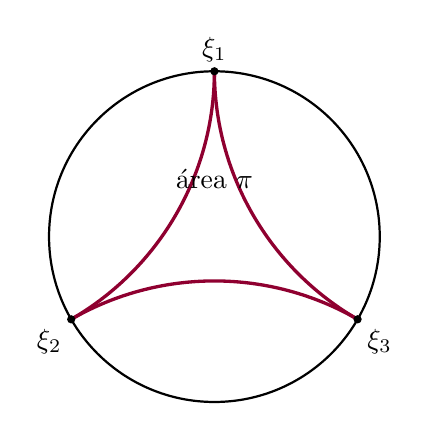
\begin{tikzpicture}[scale=2.1,line cap=round]
  \draw[thick] (0,0) circle (1cm);
  \draw[purple!75!black,very thick]
    (0,1) arc[start angle=0,end angle=-60,radius=1.7320508cm];
  \draw[purple!75!black,very thick]
    (0,1) arc[start angle=180,end angle=240,radius=1.7320508cm];
  \draw[purple!75!black,very thick]
    (-0.8660254,-0.5) arc[start angle=120,end angle=60,radius=1.7320508cm];
  \fill (0,1) circle (0.025) node[above] {$\xi_1$};
  \fill (-0.8660254,-0.5) circle (0.025) node[below left] {$\xi_2$};
  \fill (0.8660254,-0.5) circle (0.025) node[below right] {$\xi_3$};
  \node at (0,0.35) {área $\pi$};
\end{tikzpicture}
